\id{МРНТИ 06.75.07}{}

\begin{articleheader}
\sectionwithauthors{}{КУРОРТНЫЕ ЗОНЫ ТУРКЕСТАНСКОЙ ОБЛАСТИ: ОЦЕНКА МЕСТ РАЗМЕЩЕНИЯ И
ЭКОНОМИЧЕСКОЙ ЭФФЕКТИВНОСТИ}

{\bfseries
\textsuperscript{1}К.А. Омарова\textsuperscript{\envelope },
\textsuperscript{1}К.П. Мусина,
\textsuperscript{2}С.М. Рустемова,
\textsuperscript{2}Е.Б. Абеуханова
}
\end{articleheader}

\begin{affiliation}
\textsuperscript{1}ЕНУ им. Л.Н.Гумилева Астана, Казахстан,

\textsuperscript{2}КазУТБ им. К.Кулажанова Астана, Казахстан

\raggedright \textsuperscript{\envelope } Корреспондент-автор: omarova820204@mail.ru
\end{affiliation}

Статья посвящена исследованию мест размещения, расположенных в
Туркестанской и Сарыагашской курортных зонах Казахстана. В этих регионах
наблюдается рост туризма, что ставит перед гостиничным сектором задачу
повышения качества обслуживания, особенно в контексте гостиниц без
официальной категории. Важность работы заключается в анализе ключевых
показателей гостиничного бизнеса, таких как заполняемость номеров,
количество сданных номеров, средняя стоимость койко-суток. Это позволит
выявить текущие тенденции и факторы, влияющие на экономическую
эффективность мест размещения и сформулировать рекомендации для
оптимизации их функционирования.

Основной целью исследования является выявление особенностей работы
гостиниц без категории, что является актуальной проблемой для развития
туристической отрасли Казахстана. Гостиничные объекты без категории
часто не подлежат жесткому контролю качества и стандартам, что снижает
уровень обслуживания и конкуренции. Таким образом, важным аспектом
исследования является анализ факторов, влияющих на экономические
показатели гостиниц, таких как привлечение туристов, стоимость услуг,
уровень заполняемости номеров и другие параметры.

В ходе работы использованы методы статистического и сравнительного
анализа, а также экономического анализа данных, полученных от мест
размещения в Туркестанской и Сарыагашской курортных зонах. Особое
внимание уделяется сравнению экономических показателей этих регионов, с
показателями по республике, что позволяет выявить сильные и слабые
стороны функционирования гостиниц. Полученные результаты направлены на
улучшение функционирования гостиничного бизнеса и повышение
конкурентоспособности гостиниц без категорий, что, в свою очередь,
способствует улучшению качества обслуживания туристов и развитию
внутреннего туризма в Казахстане.

{\bfseries Ключевые слова:} гостиничные объекты, курортные зоны, Туркестан,
Сарыагаш, заполняемость номеров, стоимость койко-суток, гостиничные
услуги, туризм.

\begin{articleheader}
{\bfseries ТҮРКІСТАН ОБЛЫСЫНЫҢ КУРОРТТЫҚ АЙМАҚТАРЫ: ОРНАЛАСТЫРУ ОРЫНДАРЫ
ЖӘНЕ ЭКОНОМИКАЛЫҚ ТИІМДІЛІКТІ БАҒАЛАУ}

{\bfseries
\textsuperscript{1}К.А. Омарова\textsuperscript{\envelope },
\textsuperscript{1}К.П. Мусина,
\textsuperscript{2}С.М. Рустемова,
\textsuperscript{2}Е.Б. Абеуханова
}
\end{articleheader}

\begin{affiliation}
\textsuperscript{1}Л.Н.Гумилев атындағы ЕҰУ, Астана, Қазақстан,

\textsuperscript{2}Қ.Құлажанов атындағы ҚазТБУ, Астана, Қазақстан,

e-mail: \href{mailto:omarova820204@mail.ru}{\nolinkurl{omarova820204@mail.ru}}
\end{affiliation}

Бұл мақала Қазақстанның Түркістан және Сарыағаш курорттық аймақтарында
орналасқан орналастыру орындарын зерттеуге арналады. Бұл аймақтарда
туризмнің өсуі байқалады, бұл қонақүй секторына қызмет көрсету сапасын
арттыру міндетін қояды, әсіресе ресми санатқа ие емес қонақүйлер
контекстінде. Жұмыстың маңыздылығы қонақүй бизнесінің негізгі
көрсеткіштерін, мысалы, нөмірлердің толымдылығы, тапсырылған нөмірлер
саны, бір койканың орташа құны сияқты көрсеткіштерді талдауда. Бұл
қазіргі үрдістер мен орналастыру орындарының экономикалық тиімділігіне
әсер ететін факторларды анықтауға және олардың жұмысын оңтайландыру үшін
ұсыныстар жасауға мүмкіндік береді.

Зерттеудің негізгі мақсаты - категориясыз қонақүйлердің жұмыс
ерекшеліктерін анықтау, бұл Қазақстанның туристік саласының дамуындағы
өзекті мәселе болып табылады. Санатсыз қонақүйлер көбінесе сапа мен
стандарттарға қатаң бақылауға алынбайды, бұл қызмет көрсету деңгейін
және бәсекелестікті төмендетеді. Сондықтан зерттеудің маңызды аспектісі
- қонақүйлердің экономикалық көрсеткіштеріне әсер ететін факторларды,
мысалы, туристерді тарту, қызметтердің құны, нөмірлердің толымдылығы
деңгейі және басқа да параметрлерді талдау болып табылады.

Жұмыста Түркістан және Сарыағаш курорттық аймақтарынан алынған
орналастыру орындарының деректерін статистикалық және салыстырмалы
талдау әдістері, сондай-ақ экономикалық талдау әдістері қолданылды.
Аймақтардың экономикалық көрсеткіштерін республикалық көрсеткіштермен
салыстыруға ерекше көңіл бөлінеді, бұл қонақүйлердің жұмысын талдаудағы
күшті және әлсіз жақтарды анықтауға мүмкіндік береді. Алынған нәтижелер
қонақүй бизнесінің жұмысын жақсартуға және категориясыз қонақүйлердің
бәсекеге қабілеттілігін арттыруға бағытталған, бұл өз кезегінде
туристерге қызмет көрсету сапасын жақсартуға және Қазақстандағы ішкі
туризмнің дамуына ықпал етеді.

{\bfseries Кілт сөздер}: қонақүй объектілері, курорттық аймақтар,
Түркістан, Сарыағаш, нөмірлердің толымдылығы, төсек-тәуліктің құны,
қонақүй қызметтері, туризм.

\begin{articleheader}
{\bfseries RESORT ZONES OF TURKESTAN REGION: ASSESSMENT OF ACCOMMODATION
AND ECONOMIC EFFICIENCY}

{\bfseries
\textsuperscript{1}K.A. Omarova\textsuperscript{\envelope },
\textsuperscript{1}K.P. Musina,
\textsuperscript{2}S.M. Rustemova,
\textsuperscript{2}E.B. Abeukhanova
}
\end{articleheader}

\begin{affiliation}
\textsuperscript{1}L.N. Gumilyov ENU, Astana, Kazakhstan,

\textsuperscript{2}K. Kulazhanov KazUTB, Astana, Kazakhstan,

e-mail:omarova820204@mail.ru
\end{affiliation}

This article is dedicated to the study of accommodation facilities
located in the resort zones of Turkestan and Saryagash in Kazakhstan.
These regions are experiencing growth in tourism, which presents a
challenge for the hotel sector to improve service quality, especially in
the context of hotels without official classification. The importance of
this work lies in the analysis of key indicators of the hotel business,
such as room occupancy, the number of rooms rented, and the average cost
per bed-night. This will help identify current trends and factors
affecting the economic efficiency of accommodation facilities and
formulate recommendations for optimizing their operation.

The main objective of the research is to identify the characteristics of
the operation of non-classified hotels, which is a relevant issue for
the development of the tourism industry in Kazakhstan. Non-classified
hotels often do not undergo strict quality control and standards, which
reduces the level of service and competition. Thus, an important aspect
of the research is the analysis of factors affecting the economic
performance of hotels, such as attracting tourists, service costs, room
occupancy rates, and other parameters.

The study used statistical and comparative analysis methods, as well as
economic data analysis obtained from accommodation facilities in the
Turkestan and Saryagash resort zones. Special attention is given to
comparing the economic indicators of these regions with the national
averages, allowing for the identification of the strengths and
weaknesses of hotel operations. The results aim to improve the
functioning of the hotel business and enhance the competitiveness of
non-classified hotels, which in turn will contribute to improving
service quality for tourists and the development of domestic tourism in
Kazakhstan.

{\bfseries Keywords}: hotel facilities, resort zones, Turkestan, Saryagash,
room occupancy, cost per bed-night, hotel services, tourism.

\begin{multicols}{2}
{\bfseries Введение.} Актуальность выбранной темы исследования определяется
быстро развивающимся туристическим сектором Казахстана, особенно в
курортных зонах. Курортные зоны Туркестанской области имеют большой
туристский потенциал благодаря историческим и природным
достопримечательностям, однако они сталкиваются с рядом проблем в сфере
гостиничного обслуживания.

В курортных зонах Туркестанской области (Туристская зона Туркестан и
Сарыагашская курортная зона) отсутствуют гостиницы с категориями, места
размещения представлены только гостиницами без категорий и прочими
местами размещения, поэтому в дальнейшем при рассмотрении курортной зоны
Туркестанской области, мы будем использовать только эти 2 категории
размещения. Гостиницы без официальной категории, прочие места размещения
затрудняют контроль качества и стандартизацию услуг, а также снижает
привлекательность этих объектов для туристов. В связи с этим возникает
необходимость проведения анализа мест размещения без категорий, прочих
мест размещения с целью выявления факторов, влияющих на их экономическую
эффективность, таких как заполняемость номеров, стоимость койко-суток и
средняя стоимость койко-суток.

Выбор темы обусловлен отсутствием достаточного количества исследований,
посвященных именно гостиничным объектам без категории и прочим местам
размещения в курортных зонах Казахстана. Ранее работы, посвященные
гостиничной индустрии, в основном фокусировались на категориях гостиниц
и крупных туристических объектах, оставляя в тени гостиницы без
категории и прочие места размещения, которые составляют значительную
часть рынка размещения. В то же время развитие этих курортных зон
требует объективной оценки их гостиничной инфраструктуры и выявления
путей улучшения предоставляемых услуг.

Целью исследования является анализ мест размещения без категорий в
Туристской зоне Туркестан и Сарыагашской курортной зоне, оценка их
экономической эффективности и предложение рекомендаций для улучшения
качества обслуживания. Для достижения поставленной цели задачи
исследования включают анализ текущего состояния гостиничной
инфраструктуры, оценку факторов, влияющих на экономические показатели
гостиниц, а также выработку практических рекомендаций для повышения их
конкурентоспособности.

Объектом исследования является гостиничный сектор в Туристской зоне
Туркестан и Сарыагашской курортной зоне, а предметом --- гостиничные
объекты без категорий и прочие места размещения. В работе будут
использованы методы статистического и сравнительного анализа для
обработки данных о заполняемости номеров, стоимости койко-суток и других
экономических характеристик.

{\bfseries Материалы и методы.} В качестве исследовательского материала
будут использованы статистические данные, предоставленные гостиничными
объектами в Туркестанской области, а также результаты анкетирования. В
исследовании будут рассмотрены следующие ключевые показатели:
заполняемость номеров, количество сданных номеров, средняя стоимость
койко-суток.

Методы исследования включают: статистический анализ, для обработки
данных о заполняемости номеров, стоимости койко-суток и других
показателей, сравнительный анализ --- для сопоставления различных
курортных зон по республике Казахстан и выявления ключевых различий,
анализ экономических показателей --- для оценки финансовой устойчивости
мест размещения и их эффективности. В ходе исследования будут изучены
как количественные, аспекты функционирования гостиниц без категорий в
курортных зонах, что позволит более полно оценить их вклад в развитие
туризма и определить пути для повышения конкурентоспособности, также
была использована программа Power BI для составления диаграмм и анализа
данных.

{\bfseries Результаты и обсуждение.} В курортных зонах Казахстана широко
распространены небольшие, частные гостиницы без категорий,
санаторно-курортные организации, гостевые дома, апартаменты и т.д.,
которые не прошли сертификацию или не хотят тратить средства на
получение официальной категории.

Это часто встречается в развивающихся курортных зонах, где туристы
ориентируются на низкие цены и непритязательность к условиям проживания.
Множество несертифицированных объектов могут предоставлять гибкие
условия для туристов, предлагая доступные цены и меньшее количество
формальностей, что делает такие места популярными среди тех, кто ищет
бюджетное и удобное размещение {[}1{]}.

Прочие места размещения могут включать в себя такие объекты, как
турбазы, кемпинги, хостелы и частные квартиры, что также отражает
популярность нестандартных форм жилья среди туристов. Эти объекты
зачастую дешевле и не требуют официальной категории, что делает их
привлекательными для широкого круга путешественников, в том числе для
местных туристов. В последние годы в Казахстане набирает популярность
экотуризм и активный отдых, что способствует росту количества
туристических баз и прочих вариантов размещения в природных и отдаленных
местах. Эти объекты часто не поддаются сертификации по стандартам
гостиничной классификации, но предоставляют удобные условия для
специфической аудитории. Поскольку большое количество размещений без
категорий и прочих типов ориентированы на более дешевый сегмент,
предприниматели и гостиничные операторы, возможно, не видят смысла в
создании гостиниц именно с категориями, так как есть более
востребованные и прибыльные варианты (прочие места размещения, гостиницы
без категорий) {[}2{]}.

Курортные зоны представляют собой географические регионы, которые имеют
специализированную инфраструктуру для обслуживания туристов,
направленных на отдых, лечение и восстановление здоровья. Они включают
природные, климатические и культурные ресурсы, которые служат основой
для развития туристической и курортной индустрии {[}3{]}.

Касательно курортных зон всего мест размещения на период с января по
сентябрь 2024 года \- 1824 единицы, представленной в таблице 1.
\end{multicols}

{\bfseries Таблица 1 - Материально-техническая база гостиничного хозяйства
по категориям гостиниц в курортных зонах}

%% \begin{longtable}[]{@{}
%%   >{\raggedright\arraybackslash}p{(\linewidth - 14\tabcolsep) * \real{0.2007}}
%%   >{\centering\arraybackslash}p{(\linewidth - 14\tabcolsep) * \real{0.1133}}
%%   >{\centering\arraybackslash}p{(\linewidth - 14\tabcolsep) * \real{0.0973}}
%%   >{\centering\arraybackslash}p{(\linewidth - 14\tabcolsep) * \real{0.0973}}
%%   >{\centering\arraybackslash}p{(\linewidth - 14\tabcolsep) * \real{0.0973}}
%%   >{\centering\arraybackslash}p{(\linewidth - 14\tabcolsep) * \real{0.0973}}
%%   >{\centering\arraybackslash}p{(\linewidth - 14\tabcolsep) * \real{0.1596}}
%%   >{\centering\arraybackslash}p{(\linewidth - 14\tabcolsep) * \real{0.1369}}@{}}
%% \toprule\noalign{}
%% \multirow{2}{=}{\begin{minipage}[b]{\linewidth}\raggedright
%% \end{minipage}} &
%% \multirow{2}{=}{\begin{minipage}[b]{\linewidth}\centering
%% Всего
%% \end{minipage}} &
%% \multicolumn{6}{>{\centering\arraybackslash}p{(\linewidth - 14\tabcolsep) * \real{0.6859} + 10\tabcolsep}@{}}{%
%% \begin{minipage}[b]{\linewidth}\centering
%% В том числе
%% \end{minipage}} \\
%% & & \begin{minipage}[b]{\linewidth}\centering
%% 5*
%% \end{minipage} & \begin{minipage}[b]{\linewidth}\centering
%% 4*
%% \end{minipage} & \begin{minipage}[b]{\linewidth}\centering
%% 3*
%% \end{minipage} & \begin{minipage}[b]{\linewidth}\centering
%% 2*
%% \end{minipage} & \begin{minipage}[b]{\linewidth}\centering
%% Гостиница без категорий
%% \end{minipage} & \begin{minipage}[b]{\linewidth}\centering
%% Прочие места размещения
%% \end{minipage} \\
%% \midrule\noalign{}
%% \endhead
%% \bottomrule\noalign{}
%% \endlastfoot
%% Количество мест размещения, единиц & 1 824 & 11 & 23 & 6 & 2 & 602 & 1
%% 180 \\
%% Заполняемость номеров, \% & 49,8 & 72,9 & 67,3 & 71,2 & 24,5 & 44,6 &
%% - \\
%% Количество сданных номеров, единиц & 1 353 820 & 116 659 & 121 621 & 27
%% 522 & 1 941 & 651 250 & 434 827 \\
%% Средняя стоимость койко-суток, тенге & 13 957 & 65 234 & 33 832 & 25 719
%% & 16 000 & 17 462 & 11 031 \\
%% \multicolumn{8}{@{}>{\raggedright\arraybackslash}p{(\linewidth - 14\tabcolsep) * \real{1.0000} + 14\tabcolsep}@{}}{%
%% \emph{Примечание -- составлено авторами на основе данных {[}4{]}}} \\
%% \end{longtable}

\begin{multicols}{2}
В результате анализа мест размещения по курортным зонам Казахстана,
можно сделать следующие выводы: всего мест размещения в курортных зонах
рассматриваемый период с января по сентябрь 2024 года составляет 1 824
единицы, из которых распределены по категориям гостиниц следующим
образом: 5-ти звездочные гостиницы 0,6\%, 4-х звездочные - 1,\%,
3-звездочные - 0,3\%, 2-х звездочные - 0,1\%, без категорий 33\%, прочие
места размещения -- 64,7\%. Таким образом, отмечаем низкую долю
категорийных мест размещения в курортных зонах, составляющую всего 2,3\%
от общего числа, т.е. в курортных зонах наблюдается Казахстана
наблюдается недостаток крупных гостиничных объектов с высокой
категорией. Это может быть связано с нехваткой инвестиций в
строительство таких отелей, что ограничивает развитие туристической
инфраструктуры на высококачественном уровне. В курортных зонах может не
хватать спроса на высококлассные гостиницы, особенно в местах, где
основной туризм ориентирован на бюджетные варианты проживания. Это может
быть связано с тем, что туризм в Казахстане пока недостаточно развит в
плане привлечения высококлассных международных туристов, и большинство
туристов ориентируются на более дешевые варианты. Процесс сертификации
гостиниц, особенно в удаленных курортных зонах, может быть длительным и
затратным, что мешает предпринимателям и инвесторам повышать уровень
качества своих объектов и получать звезды.

Заполняемость номеров в курортных зонах Казахстана по категориям
гостиниц демонстрирует значительные различия.

5-звездочные отели предлагают высокий уровень обслуживания, удобства,
комфорт и дополнительные услуги (SPA, рестораны, бассейны, трансфер),
что привлекает более обеспеченных туристов. Это объясняет высокую
заполняемость --- такие гостиницы обычно ориентированы на туристов с
более высоким доходом, которые ценят качество и комфорт.

Эти отели часто ориентированы на международный рынок, который может быть
более стабильным и менее подверженным сезонным колебаниям.
Привлекательность высококлассных гостиниц также может объясняться их
международным признанием и известностью.5-звездочные гостиницы чаще
всего привлекают туристов с более высокими требованиями и готовы платить
за комфорт и престиж, что делает их более заполняемыми {[}5{]}.

4-звездочные отели в целом предлагают хороший уровень сервиса и
удобства, при этом цены остаются значительно ниже, чем у 5-звездочных
гостиниц. Это делает их привлекательными для более широкого круга
туристов, в том числе для среднего класса и деловых путешественников,
для туристов, которые хотят комфорт, но не готовы платить за
премиум-услуги. Это способствует хорошей заполняемости, отели могут быть
более гибкими в плане предложений для разных категорий путешественников,
что также может объяснять их стабильную заполняемость.

3-звездочные отели предлагают довольно хорошие условия за более
доступные цены. Этот сегмент привлекает массового туриста, включая
семейных путешественников и туристов с умеренным бюджетом, стремятся
предложить сбалансированный уровень качества и цен, что способствует их
высокой заполняемости, особенно в пик туристического сезона.

2-звездочные гостиницы часто предлагают минимальные условия, которые
могут не удовлетворять потребности более требовательных туристов. Низкий
уровень заполняемости может быть связан с ограниченным сервисом и
неудобствами, такими как отсутствие дополнительных услуг. Гостиницы
ориентированы на бюджетных туристов, но из-за ограниченности удобств и
сервиса могут не привлекать большое количество клиентов. В курортных
зонах, где доступны более качественные варианты туристы могут выбирать
другие отели с лучшим соотношением цены и качества, что снижает
заполняемость 2-звездочных отелей {[}6{]}.

Множество гостиниц без категории в курортных зонах могут включать в себя
частные гостиницы, санаторно-курортные организации, гостевые дома,
апартаменты и другие непрофессионально сертифицированные объекты. Такие
места зачастую предоставляют низкие цены и гибкие условия, но не всегда
обеспечивают высокий уровень сервиса. Гостиницы без категорий часто
предлагают доступные тарифы, что привлекает туристов с ограниченным
бюджетом, особенно в низкий сезон. Это может объяснять умеренную их
заполняемость, однако несмотря на доступные цены, туристы, особенно
международные, могут не предпочитать такие объекты из-за отсутствия
стандартов и предсказуемости качества обслуживания.

По поводу количества сданных номеров по курортным зонам Казахстана за
период с января по сентябрь 2024 года, можно сделать следующий анализ:
5-ти звездочные гостиницы составляют 8,6\%, 4-х звездочные -- 8,9\%, 3-х
звездочные - 2\%, гостиницы без категорий -- 48,1\%, прочие места
размещения -- 32,1\%. Несмотря на высокий уровень сервиса, 5-ти
звездочные гостиницы составляют меньшую часть всего рынка (в процентном
отношении). Их меньше по численности, но они обладают высокой
заполняемостью в сезоны пиковой активности, что и объясняет количество
сданных номеров (116 659). Заполняемость таких отелей также может быть
связана с ростом интереса к Казахстану как туристическому направлению.

4-х звездочные гостиницы предлагают высококачественные условия, что
делает их привлекательными для более широкого круга туристов, включая
как местных, так и международных, что также способствует их высокой
активности и числу сданных номеров (121~621).

3-х звездочные гостиницы предлагают хороший уровень качества за
умеренную цену, на их долю приходится меньшее количество сданных номеров
по сравнению с более дорогими гостиницами, так как туристы могут
выбирать более бюджетные варианты или альтернативные формы размещения,
(27522 номеров). Проблемы с конкуренцией со стороны гостиниц без
категорий или прочих мест размещения могут ограничивать рост сданных
номеров в этой категории.

2-х звездочные гостиницы курортных зонах Казахстана могут не
соответствовать ожиданиям более требовательных туристов из-за
ограниченных удобств и сервиса, они скорее ориентированы на местных
путешественников с ограниченным бюджетом, поэтому низкий уровень спроса
на 2-х звездочные гостиницы связан с тем, что более дешевые варианты
предоставляют аналогичные условия за меньшую цену, что снижает спрос на
отели низкой категории, (1941 номер).

В курортных зонах Казахстана широко распространены гостиницы без
категории, такие как гостевые дома, мини-отели и апартаменты,
санаторно-курортные организации. Эти объекты размещения обычно
ориентированы на бюджетных туристов, а их высокое количество сданных
номеров связано с доступностью и невысокой ценой, гибкими условиями, что
способствует увеличению числа сданных номеров, (651250).

Прочие места размещения могут включать такие объекты, как турбазы,
кемпинги, хостелы, апартаменты и другие формы жилья. Эти объекты обычно
дешевле, чем традиционные гостиницы, и привлекают разнообразные
категории туристов, что объясняет значительное количество сданных
номеров в данной категории, (434827).

По средней стоимости койко-суток 5-звездочные отели имеют самую высокую
среднюю стоимость койко-суток (65 234 тенге), что отражает их высокий
уровень сервиса и инфраструктуры.4-звездочные и 3-звездочные отели
имеют цену ниже (33 832 и 25 719 тенге соответственно), что делает их
доступными для более широкой аудитории. Гостиницы без категорий (17 462
тенге) и прочие места размещения (11 031 тенге) ориентированы на
туристов с ограниченным бюджетом.

Среди мест размещения в курортных зонах нами были изучены 2 типа
размещений: гостиницы без категорий и прочие места размещений, так как в
курортных зонах Туркестанской области отсутствуют гостиницы с
категориями звезд.
\end{multicols}

{\bfseries Таблица 2 - Основные показатели мест размещения по Республике
Казахстан и курортным зонам Туркестанской области по состоянию на первые
полугодия с 2021 - 2024гг.}

%% \begin{longtable}[]{@{}
%%   >{\raggedright\arraybackslash}p{(\linewidth - 8\tabcolsep) * \real{0.4195}}
%%   >{\centering\arraybackslash}p{(\linewidth - 8\tabcolsep) * \real{0.1497}}
%%   >{\centering\arraybackslash}p{(\linewidth - 8\tabcolsep) * \real{0.1457}}
%%   >{\centering\arraybackslash}p{(\linewidth - 8\tabcolsep) * \real{0.1457}}
%%   >{\centering\arraybackslash}p{(\linewidth - 8\tabcolsep) * \real{0.1393}}@{}}
%% \toprule\noalign{}
%% \begin{minipage}[b]{\linewidth}\raggedright
%% {\bfseries Курортные зоны}
%% \end{minipage} & \begin{minipage}[b]{\linewidth}\centering
%% {\bfseries 2021}
%% \end{minipage} & \begin{minipage}[b]{\linewidth}\centering
%% {\bfseries 2022г.}
%% \end{minipage} & \begin{minipage}[b]{\linewidth}\centering
%% {\bfseries 2023г.}
%% \end{minipage} & \begin{minipage}[b]{\linewidth}\centering
%% {\bfseries 2024г.}
%% \end{minipage} \\
%% \midrule\noalign{}
%% \endhead
%% \bottomrule\noalign{}
%% \endlastfoot
%% {\bfseries Гостиницы без категорий} & 522 & 588 & 588 & 600 \\
%% \multicolumn{5}{@{}>{\raggedright\arraybackslash}p{(\linewidth - 8\tabcolsep) * \real{1.0000} + 8\tabcolsep}@{}}{%
%% Среди них:} \\
%% Туристская зона Туркестан & 31 & 39 & 40 & 48 \\
%% Сарыагашская курортная зона & 20 & 21 & 20 & 18 \\
%% {\bfseries Прочие места размещения} & 927 & 988 & 995 & 1092 \\
%% \multicolumn{5}{@{}>{\raggedright\arraybackslash}p{(\linewidth - 8\tabcolsep) * \real{1.0000} + 8\tabcolsep}@{}}{%
%% Среди них:} \\
%% Туристская зона Туркестан & 7 & 17 & 18 & 17 \\
%% Сарыагашская курортная зона & - & - & - & - \\
%% {\bfseries Заполняемость номеров, \%} & 24,1 & 32,6 & 37,9 & 39,3 \\
%% \multicolumn{5}{@{}>{\raggedright\arraybackslash}p{(\linewidth - 8\tabcolsep) * \real{1.0000} + 8\tabcolsep}@{}}{%
%% Среди них:} \\
%% Туристская зона Туркестан & 33,1 & 28,0 & 18,9 & 22,2 \\
%% Сарыагашская курортная зона & 24,9 & 23,2 & 26,3 & 34,6 \\
%% {\bfseries Средняя стоимость койко-суток, тенге} & 9451 & 11008 & 12974 &
%% 14804 \\
%% \multicolumn{5}{@{}>{\raggedright\arraybackslash}p{(\linewidth - 8\tabcolsep) * \real{1.0000} + 8\tabcolsep}@{}}{%
%% Среди них:} \\
%% Туристская зона Туркестан & 7688 & 8027 & 10216 & 8955 \\
%% Сарыагашская курортная зона & 5567 & 6189 & 6779 & 7062 \\
%% \multicolumn{5}{@{}>{\raggedright\arraybackslash}p{(\linewidth - 8\tabcolsep) * \real{1.0000} + 8\tabcolsep}@{}}{%
%% \emph{Примечание - составлено авторами на основе данных} {[}7{]},
%% {[}8{]}, {[}9{]}, {[}10{]}.} \\
%% \end{longtable}

\begin{multicols}{2}
По данным таблицы, нами составлены диаграммы с помощью программы
\emph{Power BI}

Республики Казахстан и курортных зон Туркестанской области были
использованы данные за период первой половины 2021 -- первой половины
2024 гг.

Анализируя рисунок 1, приходим к следующим выводам: по курортным зонам
Казахстана в период с первой половины 2021 года по первую половину 2022
года наблюдается рост гостиниц без категорий на 12,6\%, в период с
первой половины 2022 года до первой половины 2023 года снижение на
5,1\%, и в период с первой половины 2023 года до первой половины 2024
года рост на 7,5\%. Общий рост по курортным зонам Казахстана с 2021 по
2024 год составил {\bfseries 14.94\%.}
\end{multicols}

\begin{figure}[H]
	\centering
	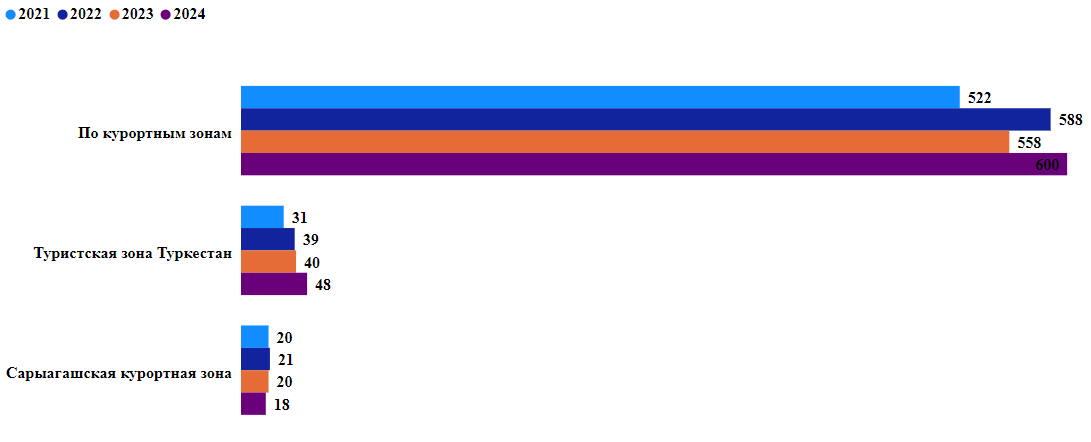
\includegraphics[width=0.8\textwidth]{media/ekon/image3}
	\caption*{Рис.1 - Гостиницы без категорий, единицы}
	\caption*{\emph{Примечание - Составлено авторами с помощью программы Power BI}}
\end{figure}

\begin{multicols}{2}
По туристской зоне Туркестан: в период с первой половины 2021 по первую
половину 2024 года наблюдается динамика роста гостиниц без категорий на
54,84\%. С периода первой половины 2021 года по первую половину 2022
года, рост составил 25,8\%, в период с первой половины 2022 года по
первую половину 2023 года -- 2,6\%, с первой половины 2023 до первой
половины 2024 года -- 20\%. Гостиницы без категорий Туристской зоны
Туркестан составляли в первой половине 2021 года, 5,9\% общего
количества гостиниц без категорий в курортных зонах, к первой половине
2024 года стали составлять 8\%.

По Сарыагашской курортной зоне в период с первой половины 2021 года по
первую половину 2024 года количество гостиниц без категорий, показывает
противоречивые показатели снижение на 10\%: с первой половины 2021 года
по первую половину 2022 года -- рост на 5\%, с периода первой половины
2022 года по первую половину 2023 года -- уменьшение на 4,8\%, с первой
половины 2023 года по первую половину 2024 года снижение на 10\%.
Гостиницы без категорий Сарыагашской курортной зоны относительно
курортных зон Казахстана в первой половине 2021 года составляли 3,8\% и
2024 годах составляют 3\%.

Таким образом доля гостиниц без категорий курортных зон Туркестанской
области, относительно курортов Казахстана составляла в первой половине
2021 года -- 9,8\%, в первой половине 2024 года 11\%, увеличив долю на
1,2\%.

По прочим местам размещения по показателям страны за период первой
половины 2021 по первую половину 2024 года, отмечается рост, с 907
единиц до 1092 единицы, (17,8\%), по курортам Туркестанской области в
Сарыагашской курортной зоне отсутствуют прочие места размещения, данные
представлены только Туристской зоной Туркестан, где рост с первой
половины 2020 года до первой половины 2024 года составил 1 единицу
(0,5\%), доля Туристской зоны Туркестан в показателях Республики
Казахстан составила в первой половине 2020 года и первой половине 2024
года (1,5\%).
\end{multicols}

\begin{figure}[H]
	\centering
	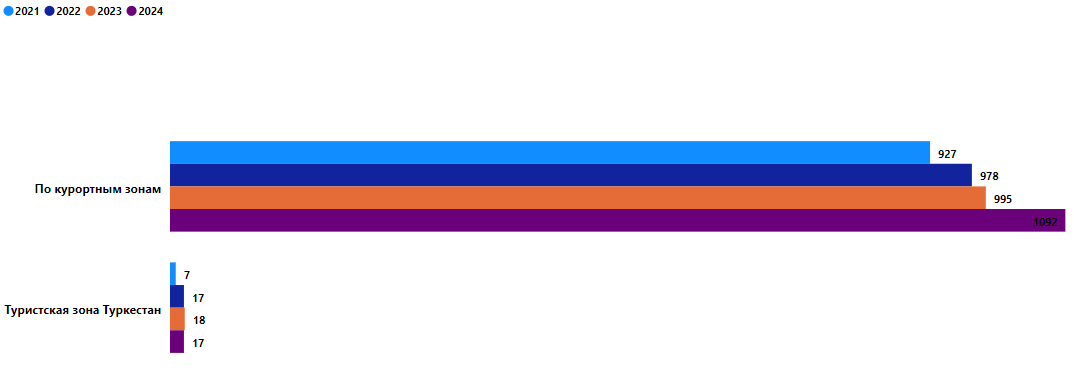
\includegraphics[width=0.8\textwidth]{media/ekon/image4}
	\caption*{Рис.2 - Прочие места размещения, единицы}
	\caption*{\emph{Примечание - Составлено авторами с помощью программы Power BI}}
\end{figure}

\begin{multicols}{2}
Следуя данным таблицы 2 и рисунка 2, можно прийти к следующим выводам,
прочие места размещения в курортных зонах Казахстана в период с первой
половины 2021 года по первую половину 2024 года имеют постоянную
положительную динамику, рост на 17,8\%. С первой половины 2021 года по
первую половину 2022 года рост составил 5,5\%, с периода первой половины
2022 года по первую половину 2023 года, рост -- 1,7\%, с первой половины
2023 по первую половину 2024 года, рост составил 9,7\%,

Прочие места размещения в Туристской зоне Туркестан в период с первой
половины 2021 по первую половину 2022 года рост составил 142\%, в период
с первой половины 2022 года по первую половину 2023 года, рост 5,9\%, с
первой половины 2023 года по первую половину 2024 года снижение на
5,6\%, общий рост с первой половины 2021 по первую половину 2024 года
составил 142,9\%. Доля Туристской зоны Туркестан к курортным зонам
Казахстана в первой половине 2021 года составила 0,75\%, в 2024 году
1,56\%, увеличив позиции на 0,81\%.

Заполняемость номеров является важным показателем деятельности мест
размещения, показывает оценку производительности мест проживания,
финансовой стабильности мест проживания и уровень привлекательности,
популярности для клиентов.
\end{multicols}

\begin{figure}[H]
	\centering
	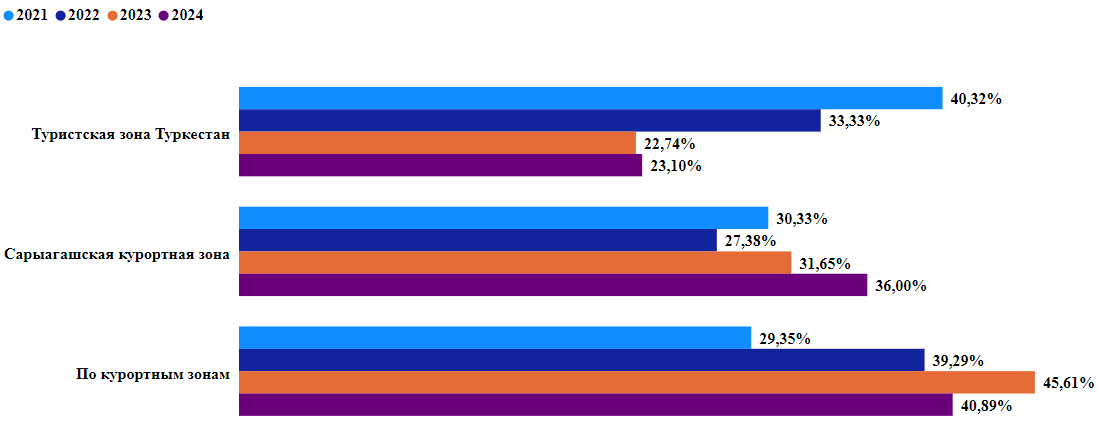
\includegraphics[width=0.8\textwidth]{media/ekon/image5}
	\caption*{Рис.3.-Заполняемость номеров, \%}
	\caption*{\emph{Примечание - Составлено авторами с помощью программы Power BI}}
\end{figure}

\begin{multicols}{2}
На основании таблицы 2 и рисунка 3, можно сделать следующие выводы:
заполняемость в курортных зонах Казахстана в период с первой половины
2021 года по первую половину 2024 года составила 55,5\%, что показывает
рост популярности среди туристов, улучшение инфраструктуры, развитие
санаториев и курортов. Заполняемость курортных зон Казахстана
демонстрирует положительную динамику, что связано с учетом пандемии
COVID-19 и ограничений на международные поездки, большое число туристов
вернулось к исследованию своих стран, ремонт и модернизация старых
объектов, строительство новых гостиниц, удобная транспортная
доступность, а также из-за стремления людей улучшить здоровье и посетить
лечебно-оздоровительные курорты.

По Туристской зоне Туркестан заполняемость номеров с периода первой
половины 2021 года по первую половину 2024 года, снизилось и составило
42,7\%. Возможно, это связано перенаправлением туристов в другие
регионы, к примеру в Сарыагашскую курортную зону, а также
инфраструктурные и сервисные проблемы, невысокий уровень обслуживания
могли привести к снижению привлекательности региона для туристов.

По Сарыагашской курортной зоне заполняемость мест размещения в курортных
зонах с первой половины 2021 по первую половину 2024 года составил
18,7\%, осуществлялся стабильный рост, после снижения в первой половине
2022 года, причиной могут быть популярность санаторно-курортных
организаций и увеличение числа посетителей данных организаций.
Сарыагашская зона стабильно улучшает свои показатели, оставаясь
востребованной у туристов, имеет хороший имидж в сфере
лечебно-оздоровительного туризма, популяризация интереса к санаторному
лечению, особенно в условиях растущего спроса на восстановление после
болезней и профилактические курсы. Сарыагашская курортная зона
пользуется популярностью среди жителей Казахстана, благодаря доступным
ценам и хорошей медицинской базе.

Средняя стоимость мест проживания постоянно должна увеличиваться в связи
с ежегодным ростом инфляции, ростом издержек на содержание мест
размещения, и сохраняющимся спросом среди посетителей. На рост цен
влияет увеличение внутреннего спроса на курорты Казахстана и
популярность внутреннего туризма, улучшением качества услуг, расширение
инфраструктуры и комфортности проживания для туристов.
\end{multicols}

\begin{figure}[H]
	\centering
	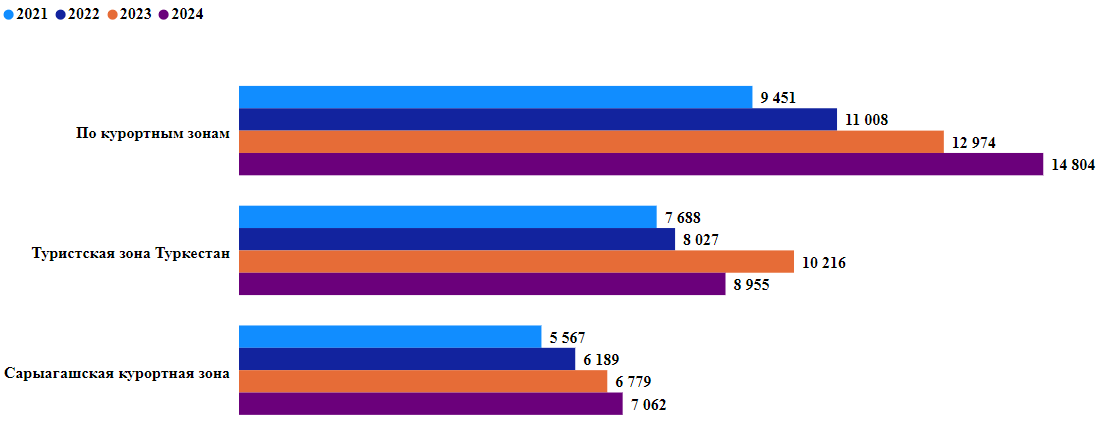
\includegraphics[width=0.8\textwidth]{media/ekon/image6}
	\caption*{Рис.4. - Средняя стоимость койко-суток, тенге}
	\caption*{\emph{Примечание - Составлено авторами с помощью программы Power BI Desktop}}
\end{figure}

\begin{multicols}{2}
Согласно данным таблицы 2 и рисунка 4, следует: процентное изменение
средней стоимости койко-суток в местах размещения по курортным зонам
Казахстана за период первой половины 2021 по первую половину 2022 года
рост цен составил 16,4\%, в первых половинах 2022 -- 2023 годов 17,9\%,
в первой половине 2023 года -- первой половине 2024 года 14\%. Общий
рост по показателям Республики Казахстан составил -- 56,3\%.

По Туристской зоне Туркестан за рассматриваемый период первой половины
2021 -- первой половины 2024 года отмечается незначительный рост цен на
места размещения на 16\%, в период первой половины 2021- первой половины
2022 года -- 4,4\%, в период первой половины 2022 года - первой половины
2023 года -- 27,7\%, резкий рост цен возможен из-за восстановления
туристского потока после пандемии и повышенным спросом на услуги, в
период первой половины 2023 -- первой половины 2024 года снижение цен на
12,4\%, что связано с падением популярности и заполняемости,
перенаправление туристского потока и осуществлено с целью притока
туристов.

В Сарыагашской курортной зоне отмечается рост цен в местах размещения в
период с первой половины 2021 года по период первой половины 2024 года,
на 26,9\% т.е. стабильный рост цен, к чему повлекла популярность и спрос
на услуги лечебно-оздоровительного туризма, повышение качества
оказываемых услуг. За период первой половины 2021 года по период первой
половины 2022 года -- на 11,2\%, в период первой половины 2022 года по
период перовой половины 2023 года -- на 9,5\%, за период с первой
половины 2023 по период первой половины 2024 года -- на 4,2\%.

{\bfseries Выводы.} Исследование мест размещения без категорий в курортных
зонах Туркестан и Сарыагаш позволило выявить ключевые проблемы и
возможности, связанные с функционированием гостиничного сектора в этих
регионах. Основными факторами, влияющими на экономическую эффективность
гостиниц, являются заполняемость номеров, стоимость койко-суток и
отсутствие стандартизации качества обслуживания. Результаты исследования
могут быть использованы для разработки рекомендаций по улучшению
инфраструктуры и повышения конкурентоспособности гостиниц в курортных
зонах.

Инфраструктура курортных зон в Казахстане представляет собой
разнообразие мест размещения, где основная масса --- это прочие места
размещения и гостиницы без категорий. Высококатегорийные гостиницы имеют
хороший уровень заполняемости и соответствующие цены, что делает их
привлекательными для туристов с более высокими доходами. Высокая
заполняемость гостиниц высококатегорийных гостиниц (от 67\% до 72\%)
свидетельствует о наличии стабильного спроса на качественное размещение,
причем отели обеспечивают хороший баланс цены и качества для различных
типов туристов.

Заполняемость курортных зон Казахстана в целом увеличивается, что
подтверждает положительные тренды для внутреннего туризма и развития
курортных инфраструктур. Туристская зона Туркестан теряет популярность,
что требует серьезного анализа причин и принятия мер для восстановления
интереса. Сарыагашская зона стабильно улучшает свои показатели,
оставаясь востребованной для туристов, особенно благодаря своему
санаторно-курортному потенциалу и лечебно-оздоровительному направлению
среди туристов, гибкой ценовой политике.

Для повышения конкурентоспособности курортных зон, привлечения
туристского потока и обеспечения устойчивого роста гостиничного бизнеса
в Туркестанской области (Сарыагашской курортной зоны и Туристской зоны
Туркестан) мы предлагаем следующие рекомендации:

- развивать и сертифицировать дополнительные высококатегорийные
гостиницы, улучшая условия для зарубежных туристов и поддерживая
внутренний рынок;

- упрощение получения категорий для малых объектов размещения;

- создавать более разнообразные ценовые категории для разных групп
туристов;

- аудит инфраструктуры и сервисного обеспечения;

- продолжить привлечение инвестиций в развитие Туркестана как
культурного и туристического центра, улучшая условия для внутреннего и
международного туризма;

- улучшение инфраструктуры;

- внедрение современных технологий;

- повышать уровень сервиса за счет привлечения высококвалифицированных
специалистов;

- совершенствовать маркетинговые кампании для привлечения туристов из
других регионов и стран, используя успешный опыт уже имеющихся курортных
зон;

- развивать уникальные курорты и санатории с акцентом на
лечебноо-оздоровительный туризм.

Таким образом, на сегодняшний день состояние рынка туристских услуг в
курортных зонах Республики Казахстан остается на удовлетворительном
уровне, необходимо обновление, совершенствование предоставления услуг,
согласно требованиям туристов, устаревание зданий, транспортной
инфраструктуры, техники, требует обновлений, контроля с государственной
позиции категорий гостиниц и других мест размещения и питания, на
уровень качества и соответствие предъявляемой категории. Вышеупомянутые
меры необходимы для повышения конкурентоспособности туристских услуг во
всех курортных зонах Казахстана.
\end{multicols}

\begin{center}
{\bfseries Литература}
\end{center}

\begin{references}
1. Губа Д.В., Воронов Ю.С. Лечебно-оздоровительный туризм: курорты и
сервис Издательство \\«Спорт», 2020, 240 с. ISBN 978-5-907225-06-0~

2. Кизимбаева А., Уразбеков А.К., Булакбай Ж.М. Влияние рынка
санаторно-курортных услуг на развитие экономики Казахстана // Вестник
ЕНУ им. Л.Н.Гумилева. - №2. -- 2024. -- С.9-26. ISSN 2789-4320

3. Salman Majeed and Woo Gon Kim Emerging trends in wellness tourism: a
scoping review // Journal of Hospitality and Tourism Insights// Emerald
Publishing Limited 2023.-Vol.6.(2) - P.853-873. DOI\\
10.1108/JHTI-02-2022-0046.

4. Статистика туризма - Места размещения в курортных зонах по типам на
январь-июнь 2024г. - {[}Электронный ресурс{]} - URL:
\href{https://stat.gov.kz/ru/industries/business-statistics/stat-tourism/}{https://stat.gov.kz}
.-Дата обращения: 26.12.2024.

5. Lina Zhong, Baolin Deng, Alastair M. Morrison, J. Andres
Coca-Stefaniak and Liyu Yang Medical, Health and Wellness Tourism
Research-A Review of the Literature (1970--2020) and Research
Agenda//\\International Journal of Environmental Research and Public
Health.- 2021.- Vol.18(20):10875. DOI \\10.3390/ijerph182010875

6. Ветитнев А.М. Лечебный туризм: учебное пособие/ А.М. Ветитнев, А.С.
Кусков - Москва: Форум, 2010.- 592 с. ISBN 978-5-91134-364-4.

7. Статистика туризма. Электронные таблицы
\href{https://stat.gov.kz/api/iblock/element/26608/file/ru/}{О
деятельности мест размещения в Республике Казахстан (январь-июнь 2021
года)} - {[}Электронный ресурс{]} - URL:
\href{https://stat.gov.kz/ru/industries/business-statistics/stat-tourism/spreadsheets/?year=2021&name}{https://stat.gov.kz}.-
Дата обращения: 20.11.2024

8. Статистика туризма. Электронные
таблицы.\href{https://stat.gov.kz/api/iblock/element/4430/file/ru/}{О
деятельности мест размещения в Республике Казахстан (Январь-июнь
2022г.)} - {[}Электронный ресурс{]} - URL:
\href{https://stat.gov.kz/ru/industries/business-statistics/stat-ourism/spreadsheets/?year=2022&name}{https://stat.gov.kz}.-Дата
обращения: 22.11.2024.

9. Статистика туризма. Электронные таблицы. О деятельности мест
размещения в Республике Казахстан (январь-июнь 2023г.) - {[}Электронный
ресурс{]} - URL:
\href{https://stat.gov.kz/ru/industries/business-statistics/stat-tourism/spreadsheets/?year=2023&name}{https://stat.gov.kz}.-
Дата обращения: 23.11.2024.

10. Статистика туризма. Электронные таблицы. О деятельности мест
размещения в Республике Казахстан (январь-июнь 2024г.) - {[}Электронный
ресурс{]} - URL:
\href{https://stat.gov.kz/ru/industries/business-statistics/stat-tourism/spreadsheets/?year=2024&name}{https://stat.gov.kz}.-
Дата обращения: 25.11.2024.
\end{references}

\begin{center}
{\bfseries References}
\end{center}

\begin{references}
1. Guba D.V., Voronov Ju.S. Lechebno-ozdorovitel' nyj
turizm: kurorty i servis Izdatel' stvo «Sport», 2020, 240
s. ISBN 978-5-907225-06-0. {[}in Russian{]}

2. Kizimbaeva A., Urazbekov A.K., Bulakbaj Zh.M. Vlijanie rynka
sanatorno-kurortnyh uslug na razvitie jekonomiki Kazahstana // Vestnik
ENU im. L.N.Gumileva. - №2. -- 2024. -- S.9-26. ISSN 2789-4320. {[}in
Russian{]}

3. Salman Majeed and Woo Gon Kim Emerging trends in wellness tourism: a
scoping review // Journal of Hospitality and Tourism Insights// Emerald
Publishing Limited 2023.-Vol.6.(2) - P.853-873. DOI\\
10.1108/JHTI-02-2022-0046.

4. Statistika turizma - Mesta razmeshhenija v kurortnyh zonah po tipam
na janvar'-ijun'{} 2024g. - Jelektronnyj
resurs - URL:
https://stat.gov.kz/ru/industries/business-statistics/stat-tourism/
.-Data obrashhenija: \\26.12.2024 {[}in Russian{]}

5. Lina Zhong, Baolin Deng, Alastair M. Morrison, J. Andres
Coca-Stefaniak and Liyu Yang Medical, Health and Wellness Tourism
Research-A Review of the Literature (1970--2020) and Research
Agenda//International Journal of Environmental Research and Public
Health.- 2021.- Vol.18(20):10875. DOI 10.3390/ijerph182010875

6. Vetitnev A.M. Lechebnyj turizm: uchebnoe posobie/ A.M. Vetitnev, A.S.
Kuskov - Moskva: Forum, 2010.- 592 s. ISBN 978-5-91134-364-4. {[}in
Russian{]}

7. Statistika turizma. Jelektronnye tablicy O
dejatel' nosti mest razmeshhenija v Respublike Kazahstan
(janvar'-ijun'{} 2021 goda) - Jelektronnyj
resurs - URL:
\href{https://stat.gov.kz/ru/industries/business-statistics/stat-tourism/spreadsheets/?year=2021&name}{https://stat.gov.kz}.-
Data obrashhenija: 20.11.2024. {[}in Russian{]}

8. Statistika turizma. Jelektronnye tablicy.O
dejatel' nosti mest razmeshhenija v Respublike Kazahstan
(Janvar'-ijun'{} 2022g.) - Jelektronnyj
resurs - URL:
https://stat.gov.kz/ru/industries/business-statistics/stat-ourism/spreadsheets/?year=2022\&name.-Data
obrashhenija: 22.11.2024. {[}in Russian{]}

9. Statistika turizma. Jelektronnye tablicy. O
dejatel' nosti mest razmeshhenija v Respublike Kazahstan
(janvar'-ijun'{} 2023g.) - Jelektronnyj
resurs - URL:
https://stat.gov.kz/ru/industries/business-statistics/stat-tourism/spreadsheets/?year=2023\&name.-
Data obrashhenija: 23.11.2024. {[}in Russian{]}

10. Statistika turizma. Jelektronnye tablicy. O
dejatel' nosti mest razmeshhenija v Respublike Kazahstan
(janvar'-ijun'{} 2024g.) - Jelektronnyj
resurs - URL:
https://stat.gov.kz/ru/industries/business-statistics/stat-tourism/spreadsheets/?year=2024\&name.-
Data obrashhenija: 25.11.2024. {[}in Russian{]}
\end{references}

\begin{authorinfo}
\emph{{\bfseries Сведения об авторах}}

Омарова К.А.- докторант, Евразийский национальный университет им.
Л.Н.Гумилева, г. Астана, Казахстан, е-mail:
\href{mailto:omarova820204@mail.ru}{\nolinkurl{omarova820204@mail.ru}};
https://orcid.org/0009-0001-4434-1435

Мусина К. П. - кандидат экономических наук, ассоциированный профессор
кафедры «Туризм» Евразийский национальный университет им. Л.Н.Гумилева,
г. Астана, Казахстан, е-mail:
\href{mailto:2kamshatmussina@mail.ru}{kamshatmussina@mail.ru};
https://orcid.org0000-0002-6772-6338

Рустемова С.М. - магистр наук, сеньор-лектор кафедры «Туризм и сервис»
Казахский университет технологии и бизнеса им. К.Кулажанова Астана,
Казахстан, е-mail:
\href{mailto:sabiruwa1986@mail.ru}{\nolinkurl{sabiruwa1986@mail.ru}};\\
\url{https://orcid.org/0000-0003-1004-2135}

Абеуханова Е.Б. - магистр экономических наук, сеньор-лектор кафедры
«Туризм и сервис» Казахский университет технологии и бизнеса им.
К.Кулажанова Астана, Казахстан, е-mail:
\href{mailto:erkejana77@mail.ru}{\nolinkurl{erkejana77@mail.ru}}
\url{https://orcid.org/0009-0000-8249-4080}

\emph{{\bfseries Information about authors}}

Omarova K.A. - main author, doctoral student, L.N.Gumilyov Eurasian
National University, Astana, Kazakhstan, е-mail:
\href{mailto:omarova820204@mail.ru}{\nolinkurl{omarova820204@mail.ru}};

Musina K. P. - сandidate of Economic Sciences, Associate Professor of
the Department of Tourism, L.N.Gumilyov Eurasian National University,
Astana, Kazakhstan, е-mail: kamshatmussina@mail.ru;

Rustemova S.M. - Master of Science, Senior Lecturer of the Department
"Tourism and Service" K.Kulazhanov Kazakh University of Technology and
Business Astana, Kazakhstan, е-mail:
\href{mailto:sabiruwa1986@mail.ru}{\nolinkurl{sabiruwa1986@mail.ru}};

Abeukhanova Y.B. - Master of Economics, Senior Lecturer of the
Department of Tourism and Service, K.Kulazhanov Kazakh University of
Technology and Business Astana, Kazakhstan, е-mail:
\href{mailto:erkejana77@mail.ru}{\nolinkurl{erkejana77@mail.ru}};
\end{authorinfo}
